\item O sino de \SI{150}{\kilogram} está em repouso na posição vertical quando é atingido pela viga de madeira de \SI{37.5}{\kilogram}, suspensa por duas cordas de igual comprimento. Se a viga é solta do repouso em $\theta=\SI{45}{^{\circ}}$, determine a velocidade angular do sino e a velocidade da viga logo após o impacto. O coeficiente de restituição entre o sino e a viga é $e=0.6$. O centro de gravidade do sino está localizado no ponto $G$ e seu raio de giração em relação a $G$ é $k_{G}=\SI{.45}{\meter}$

\import{../answers}{answer-13}

\vspace{-1cm}
\begin{flushright}
	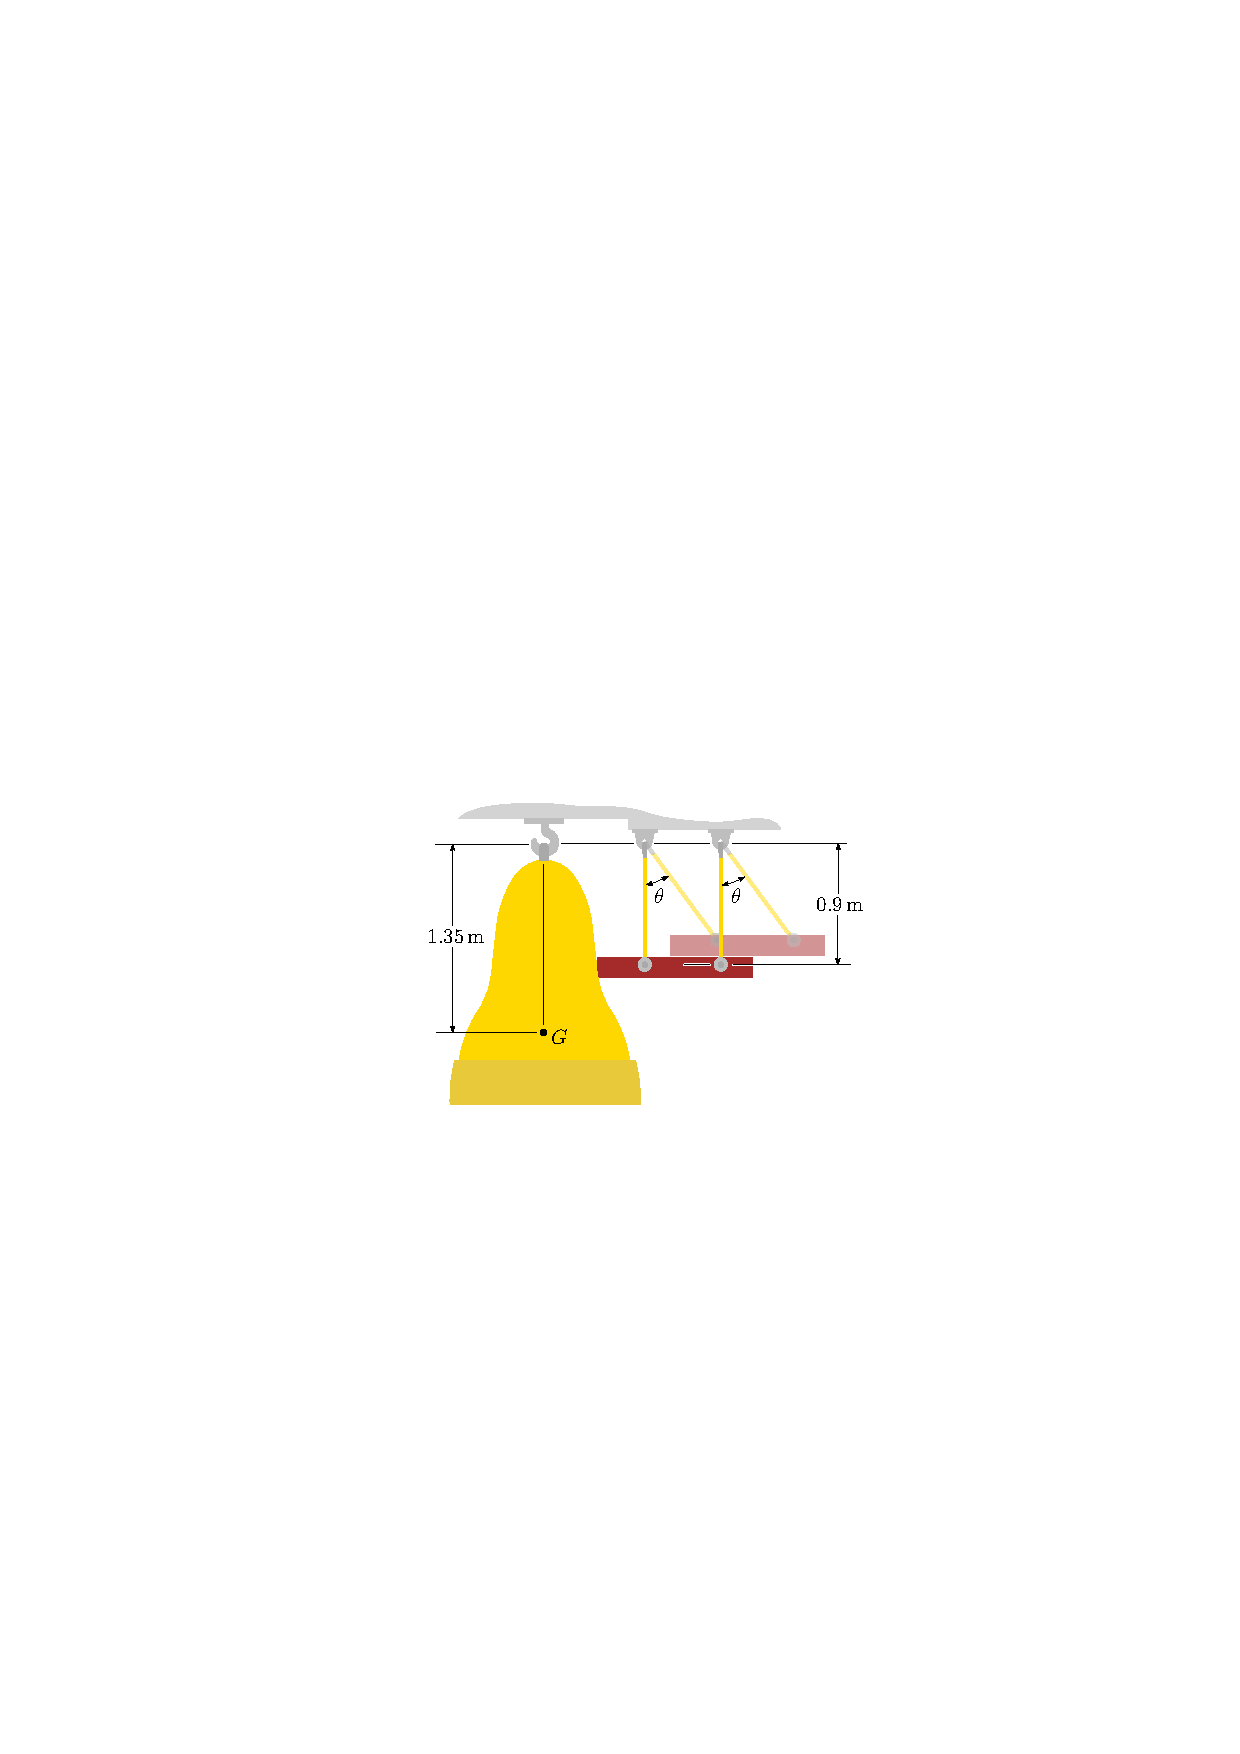
\includegraphics[scale=1.2]{../../images/draw_12}
\end{flushright}
